\documentclass{standalone}
\usepackage[usenames,dvipsnames]{xcolor}
\usepackage{tikz}
\usetikzlibrary{arrows.meta}


\begin{document}

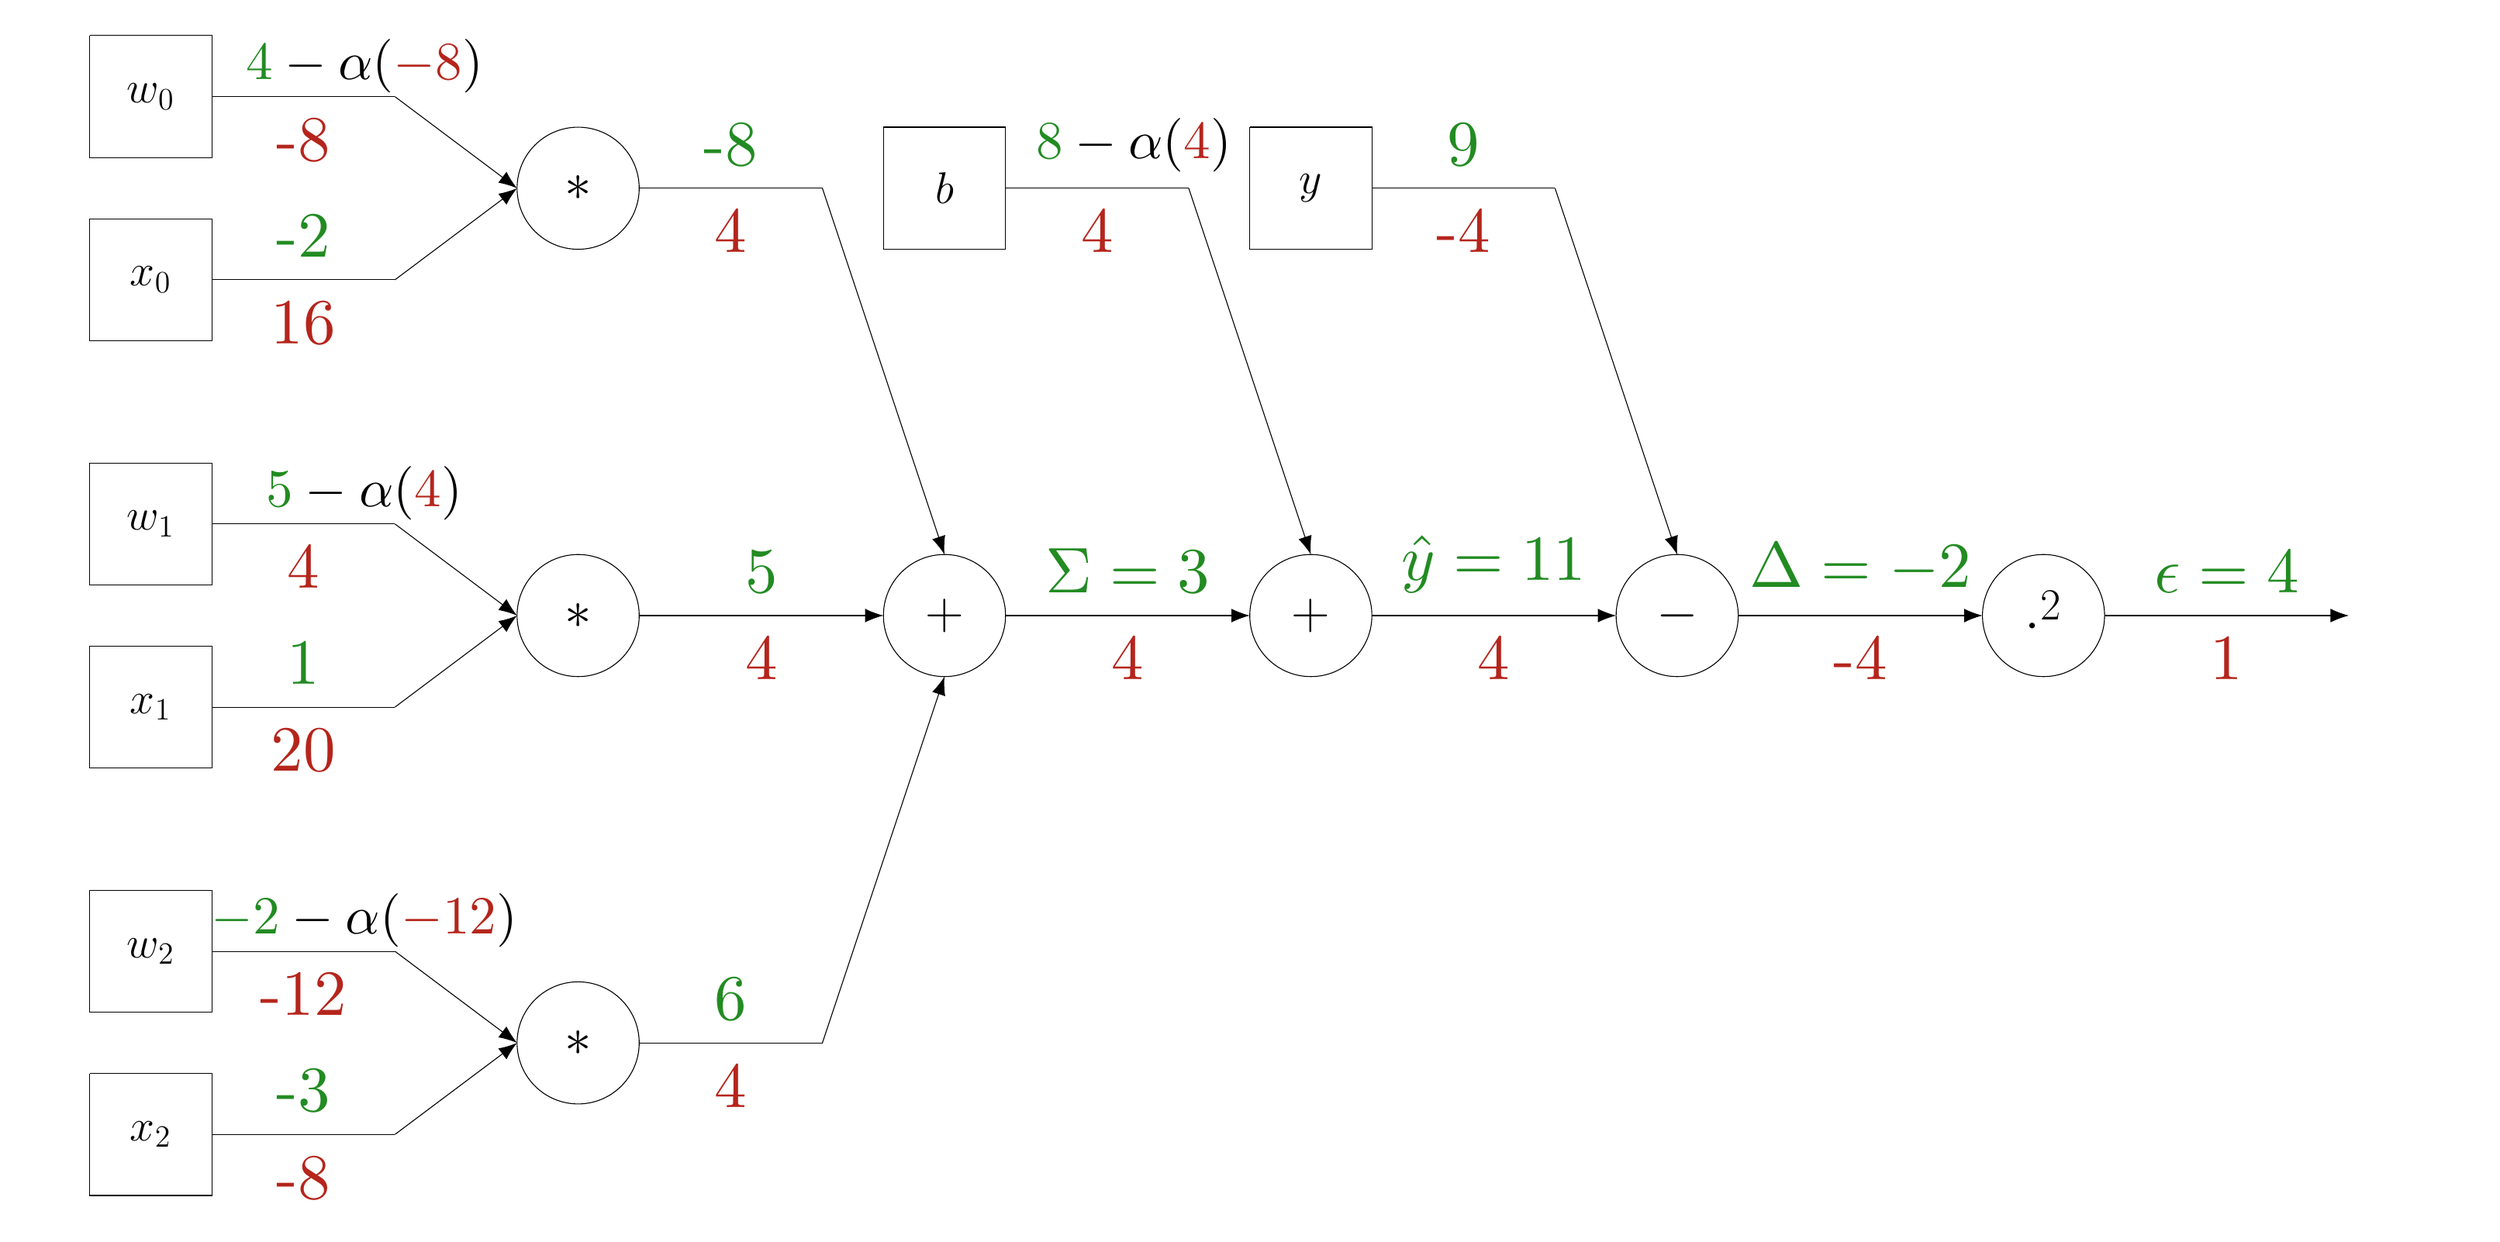
\begin{tikzpicture}

% anchor points for size
\node at (0,0) {} { };
\node at (40,19) {} { };

% w0
\draw (1,19) -- (3,19) -- (3,17) -- (1,17) -- (1,19);
\node[] at (2,18) {\huge $w_0$};

% x0
\draw (1,16) -- (3,16) -- (3,14) -- (1,14) -- (1,16);
\node[] at (2,15) {\huge $x_0$};

% op w0 * x0
\draw (9, 16.5) circle (1cm);
\node[] at (9, 16.5) {\Huge $*$}; 

% arrow from w0 to *
%\draw (3,18) -- node[above,scale=3,text=ForestGreen] {4} node[below,scale=3,text=BrickRed] {-8} (6,18);
\draw (3,18) -- node[below,scale=3,text=BrickRed] {-8} (6,18);
\node[scale=2.5] at (5.5,18.5) {$\textcolor{ForestGreen}{4}-\alpha(\textcolor{BrickRed}{-8})$};
\draw [-{Latex[length=3mm]}] (6,18) -- (8,16.5);

% arrow from x0 to *
\draw (3,15) -- node[above,scale=3,text=ForestGreen] {-2} node[below,scale=3,text=BrickRed] {16} (6,15);
\draw [-{Latex[length=3mm]}] (6,15) -- (8,16.5);


% w1
\draw (1,12) -- (3,12) -- (3,10) -- (1,10) -- (1,12);
\node[] at (2,11) {\huge $w_1$};

% x1
\draw (1,9) -- (3,9) -- (3,7) -- (1,7) -- (1,9);
\node[] at (2,8) {\huge $x_1$};

% op w1 * x1
\draw (9, 9.5) circle (1cm);
\node[] at (9, 9.5) {\Huge $*$}; 

% arrow from w1 to *
%\draw (3,11) -- node[above,scale=3,text=ForestGreen] {5} node[below,scale=3,text=BrickRed] {4} (6,11);
\draw (3,11) -- node[below,scale=3,text=BrickRed] {4} (6,11);
\node[scale=2.5] at (5.5,11.5) {$\textcolor{ForestGreen}{5}-\alpha(\textcolor{BrickRed}{4})$};
\draw [-{Latex[length=3mm]}] (6,11) -- (8,9.5);

% arrow from x1 to *
\draw (3,8) -- node[above,scale=3,text=ForestGreen] {1} node[below,scale=3,text=BrickRed] {20} (6,8);
\draw [-{Latex[length=3mm]}] (6,8) -- (8,9.5);


% w2
\draw (1,5) -- (3,5) -- (3,3) -- (1,3) -- (1,5);
\node[] at (2,4) {\huge $w_2$};

% x2
\draw (1,2) -- (3,2) -- (3,0) -- (1,0) -- (1,2);
\node[] at (2,1) {\huge $x_2$};

% op w2 * x2
\draw (9, 2.5) circle (1cm);
\node[] at (9, 2.5) {\Huge $*$}; 

% arrow from w2 to *
%\draw (3,4) -- node[above,scale=3,text=ForestGreen] {-2} node[below,scale=3,text=BrickRed] {-12} (6,4);
\draw (3,4) -- node[below,scale=3,text=BrickRed] {-12} (6,4);
\node[scale=2.5] at (5.5,4.5) {$\textcolor{ForestGreen}{-2}-\alpha(\textcolor{BrickRed}{-12})$};
\draw [-{Latex[length=3mm]}] (6,4) -- (8,2.5);

% arrow from x2 to *
\draw (3,1) -- node[above,scale=3,text=ForestGreen] {-3} node[below,scale=3,text=BrickRed] {-8} (6,1);
\draw [-{Latex[length=3mm]}] (6,1) -- (8,2.5);


% op sum(w_i * x_i)
\draw (15, 9.5) circle (1cm);
\node[] at (15, 9.5) {\Huge $+$};

% arrow from w0*x0 to sum
\draw (10,16.5) -- node[above,scale=3,text=ForestGreen] {-8} node[below,scale=3,text=BrickRed] {4} (13,16.5);
\draw [-{Latex[length=3mm]}] (13,16.5) -- (15,10.5);

% arrow from w1*x1 to sum
\draw [-{Latex[length=3mm]}] (10, 9.5) -- node[above,scale=3,text=ForestGreen] {5} node[below,scale=3,text=BrickRed] {4} (14,9.5);

% arrow from w2*x2 to sum
\draw (10,2.5) -- node[above,scale=3,text=ForestGreen] {6} node[below,scale=3,text=BrickRed] {4} (13,2.5);
\draw [-{Latex[length=3mm]}] (13,2.5) -- (15,8.5);

% op plus b

% b
\draw (14,17.5) -- (16,17.5) -- (16,15.5) -- (14,15.5) -- (14,17.5);
\node[] at (15,16.5) {\huge $b$};

% arrow from b to +b
%\draw (16,16.5) -- node[above,scale=3,text=ForestGreen] {8} node[below,scale=3,text=BrickRed] {4} (19,16.5);
\node[scale=2.5] at (18.1,17.2) {$\textcolor{ForestGreen}{8}-\alpha(\textcolor{BrickRed}{4})$};
\draw (16,16.5) -- node[below,scale=3,text=BrickRed] {4} (19,16.5);
\draw [-{Latex[length=3mm]}] (19,16.5) -- (21,10.5);


\draw (21, 9.5) circle (1cm);
\node[] at (21, 9.5) {\Huge $+$};

% arrow from sum to +b
\draw [-{Latex[length=3mm]}] (16, 9.5) -- node[above,scale=3,text=ForestGreen] {$\Sigma=3$} node[below,scale=3,text=BrickRed] {4} (20,9.5);

% arrow from +b to -y
\draw [-{Latex[length=3mm]}] (22, 9.5) -- node[above,scale=3,text=ForestGreen] {$\hat{y}=11$} node[below,scale=3,text=BrickRed] {4} (26,9.5);

% HIDE -- show which part of the computation graph gives $y_predicted$
%\node[] at (28,9.5) {\huge $y_\textnormal{predicted}$};


% y
\draw (20,17.5) -- (22,17.5) -- (22,15.5) -- (20,15.5) -- (20,17.5);
\node[] at (21,16.5) {\huge $y$};

% arrow from y to -y
\draw (22,16.5) -- node[above,scale=3,text=ForestGreen] {9} node[below,scale=3,text=BrickRed] {-4} (25,16.5);
\draw [-{Latex[length=3mm]}] (25,16.5) -- (27,10.5);



% minus y
\draw (27, 9.5) circle (1cm);
\node[] at (27, 9.5) {\Huge $-$};


% ^2
\draw (33, 9.5) circle (1cm);
\node[] at (33, 9.5) {\Huge $\cdot^2$};

% arrow from -y to square
\draw [-{Latex[length=3mm]}] (28, 9.5) -- node[above,scale=3,text=ForestGreen] {$\Delta=-2$} node[below,scale=3,text=BrickRed] {-4} (32,9.5);

% arrow out of square
\draw [-{Latex[length=3mm]}] (34, 9.5) -- node[above,scale=3,text=ForestGreen] {$\epsilon=4$} node[below,scale=3,text=BrickRed] {1} (38,9.5);

% HIDE -- error term
%\node [] at (39, 9.5) {\huge Error};

% backprop calculations
%\node at (33,6) {$$
%	f(z) = z^2
%$$}


%
% f(z) = z^2
% \frac{df}{dz} = 2z
% \frac{d\epsilon}{dz} = \frac{df}{dz} * \frac{dz}{d\epsilon} = 2(-2) * 1

% f(y, \hat{y}) = y-\hat{y}
% \frac{df}{d\hat{y}} = -1
% \frac{df}{d\

\end{tikzpicture}

\end{document}